\section{Селективное лазерное спекание}


\subsection{Технология}

\begin{figure}[h]
    \centering
    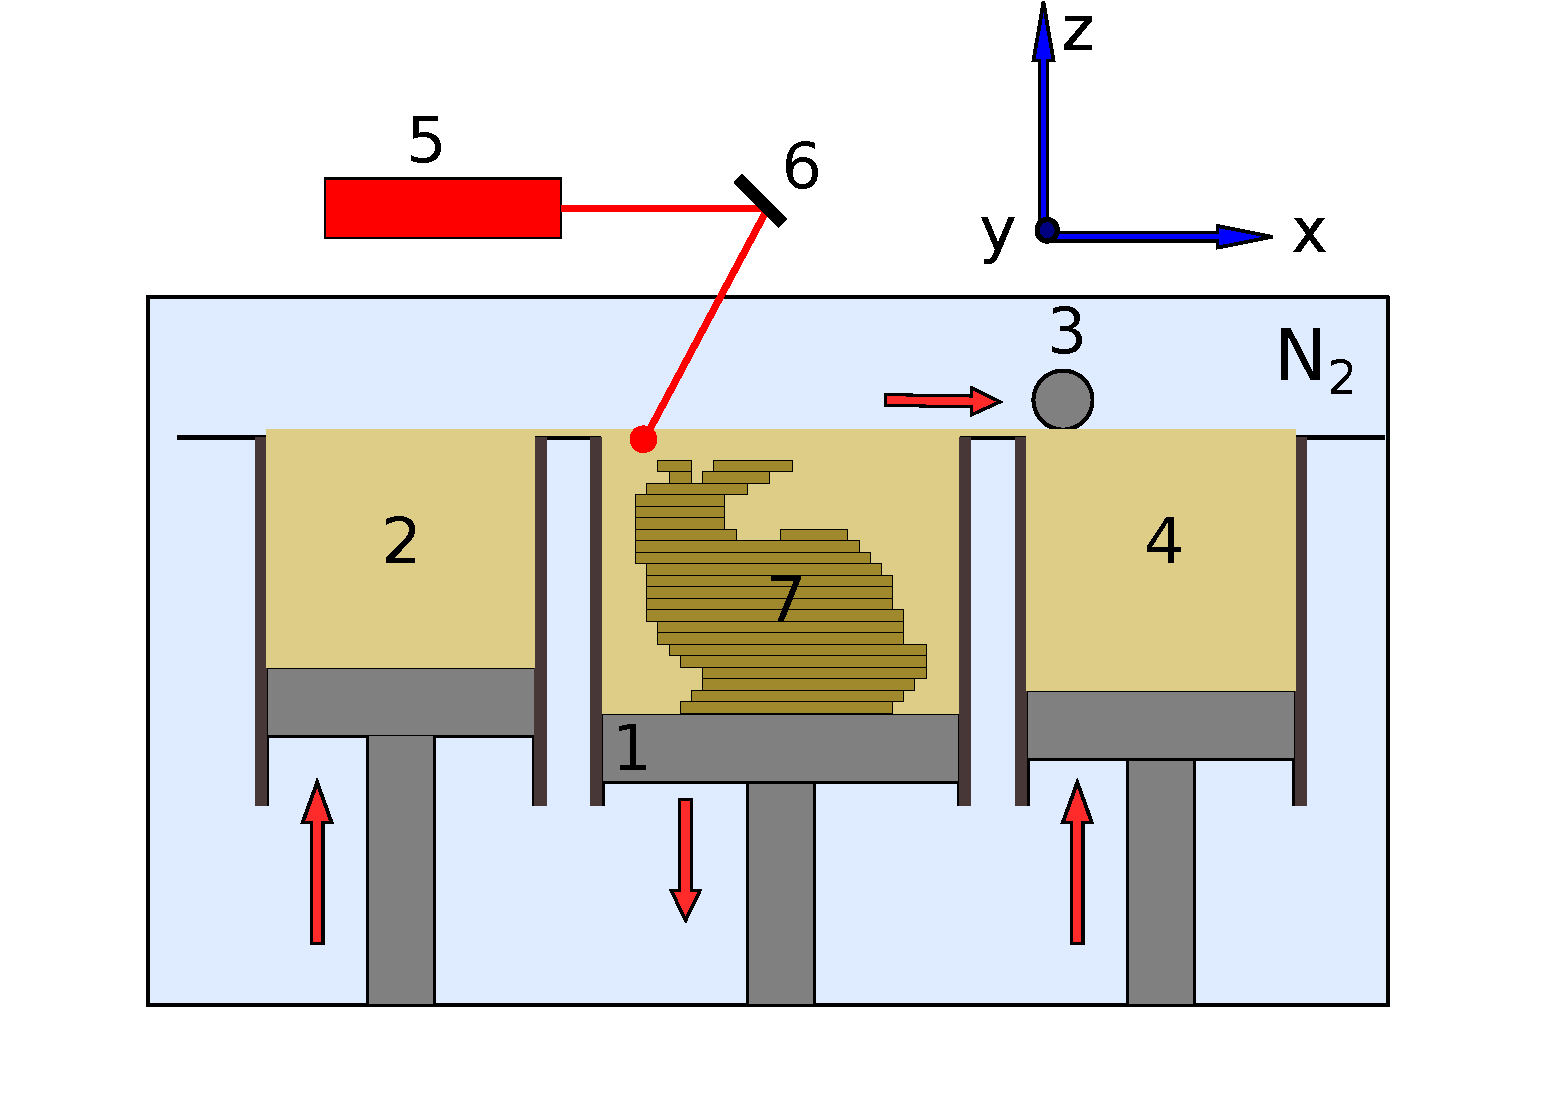
\includegraphics[width=\linewidth]{fig/sls-2d.pdf}
    \caption{[WIP]Принцип работы SLS-принтера}
    \label{fig:printer}
\end{figure}


\paragraph{Что это вообще} 
Лазерное спекание полимеров -- технология аддитивного производства.  Индивидуальные и составные части создаются напрямую из данных CAD без потребности в специфических инструментах. Материал -- полимерный порошок -- послойно распределяется и селективно плавится с помощью лазера. Напечатанная деталь остается в окружении неиспользованного порошка.
\paragraph{Общий принцип. }Процесс печати изделия изображен схематически на рис. \ref{fig:printer}.
The
feed powder hopper (1) dispenses a polymer powder into a
recoater unit (2) which moves in x direction and thereby
recoats thin powder layers onto the build platform (5). Residual
powder is collected in an overflow bin (6). After each layer, the
platform moves down in z direction. Typical layer thicknesses
are about 50 to 200 mm. During the build process, the so-called
part cake (3) “grows” from the bottom to the top. By volume,
it typically consists of about 90% unsintered (aged) powder and
of about 10% built parts (4). In each layer, the whole part cake
surface is preheated with infrared heaters (7) up to 2 to 5 K
below melting temperature of the material. The energy needed
to fully melt the powder is brought in with a CO2 laser (8) that
selectively melts the desired slice geometry. In this phase,
unmolten powder and molten parts remain quasi-isothermal
within the same layer.7 This so-called temperature window has
to be lower than the melting temperature and higher than the
recrystallization temperature of the material8 in order to prevent
warpage during the manufacturing process. Hence, heating up
the whole part cake is a prerequisite for a reliable LS process.
To reduce oxidation, the process chamber is purged with nitrogen
(residual oxygen <2%). When the build process finishes,
the part cake is first cooled down within the machine for about
10 h (nitrogen flow) and then outside of the machine until the
core temperature is below glass transition temperature. Then,
the parts are removed from the, unmolten powder. With total
build heights of up to 600 mm, typical layer thicknesses of
about 100 mm and layer times of about 10 of 40 s, the overall
manufacturing process may take many hours or even days,4
resulting in various powder ageing effects.




Polymer laser sintering (LS) is an important additive manufacturing (AM) technology. Individual and complex parts are
directly produced from CAD data without the need of specific tools. The raw material is a polymer powder, which is deposited layerwise
and melted selectively with a laser. Built parts are embedded in residual unmolten powder





\paragraph{Особенности сравнению с традиционными методами.}
Thereby, product development times can be reduced tremendously.
Other advantages are, for example, the fast and costefficient
production of low-volume, individual and complex parts
and structures.3
\paragraph{Особенности по сравнению с другой 3д-печатью.}

\subsection{Сращивание частиц порошка при СЛС}
Laser-based consolidation of 3D parts from layers of
powder material pre-deposited on a ‘build platform’ is
commonly referred to as Selective Laser Sintering (SLS)
or Selective Laser Melting (SLM). The distinction between
SLS and SLM is rough, vague and does not cover all

Классификация схематически показана на рис.\ref{fig:binding}

\begin{figure}[h]
    \centering
    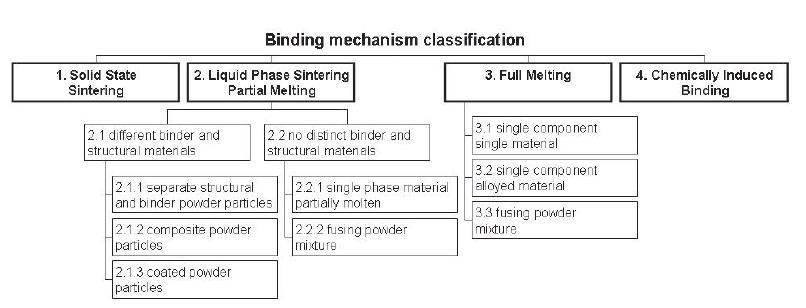
\includegraphics[width = \linewidth]{fig/binding.PNG}
    \caption{Механизмы консолидации порошка}
    \label{fig:binding}
\end{figure}

\paragraph{Симуляция процесса close-up.}


% вся инфа которая пока есть
Высокая интенсивнсть лазерного излучения позволяет быстро нагревать небольшие участки материала, создавая большие градиенты температур \cite{sls-sim2016}.
\\
Симуляция СЛС показывает, что у композитных порошков будет сильно отличное распределение температур, особенно глубина плавления. (по крайне мере в полиамидах)\cite{sls-sim2016}. Экспериментальное исследование становится эфеективнее, если есть модель процесса.
Какие нужны параметры для модели?
%%%%%%%%%%%%%%%%%%%%%%%%%%%%%%%%%%%%%%%%%%%%%%

\section{Требования к материалам для СЛС}




%вступление
The availability of suitable LS polymer powders is quite limited.
The manufacturing process requires certain polymer properties,
mainly a large process window and a low melt viscosity,4 and
particle/powder properties, for example, a good flowability and
high bulk density.9,10 Due to these limitations, the majority of
all LS applications is currently based on polyamide 12 (see Figure
2)


Конечные характеристики изделия, полученного по технологии СЛС, во многом зависят от от свойств начального порошка (морфология, размер, распределние размеров, объемная плотность, термические свойства, вязкость, поверхностное натяжение )  и параметров спекания (мощность лазера, скорость сканирования, диаметр пятна излучения лазера ).

\subsection{Механические характеристики}
первая глава из
\cite{termopols}
\subsection{Тепловые характеристики}

Built parts are embedded in residual unmolten powder, the so-called part cake, which undergoes
thermal ageing effects due to the exposure to high temperatures for long times during the manufacturing process. Hence, the
recyclability of the unmolten powder is limited. \cite{ageing}


\subsection{Морфология частиц порошка}
Морфология частиц определяет пространственное расположение частиц порошка (stacking degree) относительно друг друга. Сферические (с гладкой поверхностью) частицы имеют высокую плотность упаковки. Они обеспечивают  сыпучесть in systems of applying the material with minimal resistance. В добавок, сферические частицы хорошо связываются в процессе спекания.Показано, что 
during the transition from powder particles with predominantly spherical morphology to particles of irregular shape of the same material, the elastic modulus decreases by almost 40 \%. 
(найти ссылку ,потом перевести).
Таким образом, сферический частицы с хорошей сыпучестью и высокой плотностью упаковки представляют идеальные характеристики стартового пороша для испольщования в СЛС.\\
В то же время использование частиц неправильной формы с большой вариацией в размерах ведет к созданию продуктов с более высокими механическими характеристиками в сравнении с использованием mainle сферических частиц с узким распределением размеров.

\subsection{Кристалличность}

\subsection{Прочее}


\subsection{Полиэфиримиды ряда R-BAPB }
		
	\begin{figure}[h]
	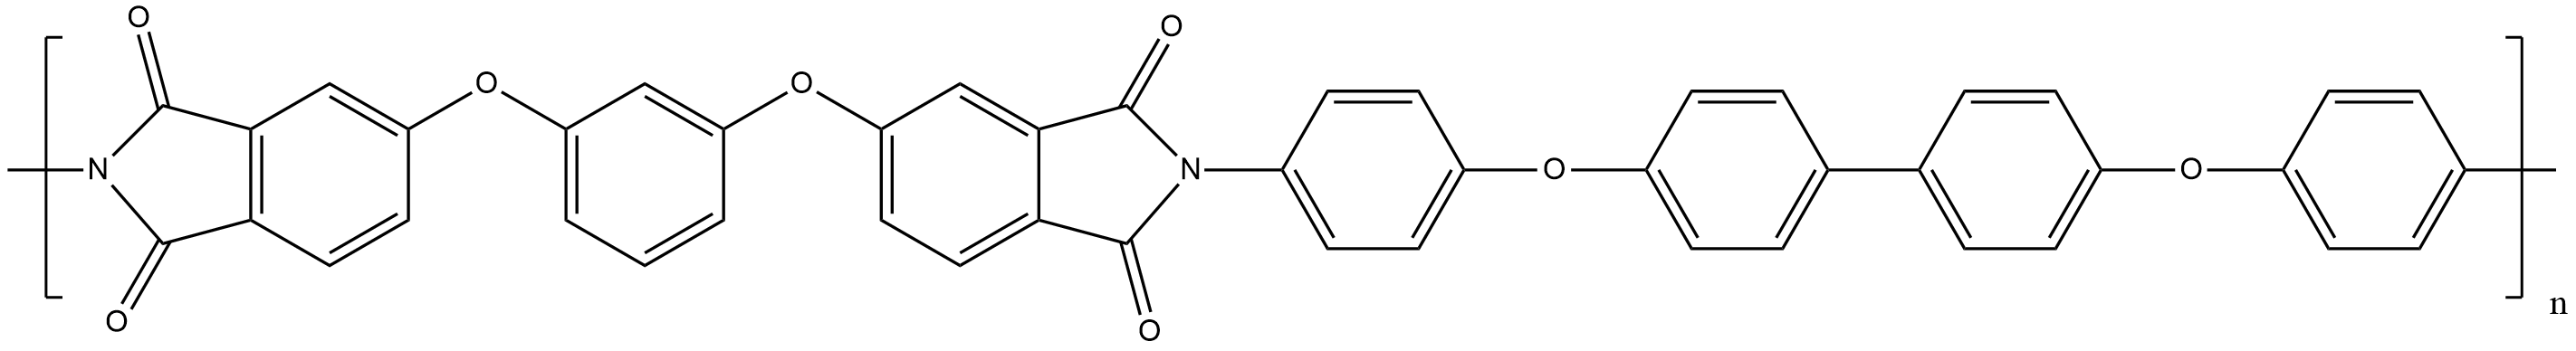
\includegraphics[width=\textwidth]{fig/formula.png}
	\caption{Структура полимера Р-ОДФО \cite{pi-formula}}
	\label{fig:formula}
	\end{figure}

Что это\\
Особенности\\
Намеренные ранее характеристики\\
Использование в промышленности\\
Композиты\\
Короче, они збс и подходят для СЛС\\
Что нужно выяснить.\\

\section{Кристаллическая структура полимеров}

Что ее характеризует
Поскольку кристаллические области в этих полимерах формируются из длинных цепей, их кристаллизация сложна и сильно чувствительа к маленьким изменениям в полимерной (compostion), добавкам, температуре и механическим воздействиям.\\
Не все полимеры кристаллизуются, а те, что кристаллизуются, редко делают это полностью: только небольшая часть crystallizable цепей incorporated into crystalline domains, а остальные segregate into amorphous domains. Степеь кристалличности и характеристики кристаллических domains являются самыми важными морфологическими характеристиками, которые определяют физические свойства такие как плотность, mechanical strength, processability, permeability and degradability частичнокристаллического полимера.\\
Степень кристалличности типичного полимера варьируется в пределах от 10 до 80 \%. Сравните с металлами, которые, за исключением металлических стекол, почти всегда полностью кристалличны, и ceramics, которые или полностью кристалличны, или аморфны.\\ \cite{cryst3} или \cite{cryst1}






Кристаллическая структура полимеров менее идеальна чем кристаллы соединений с меньшей молекулярной массой. Как правило полимерные материалы находятся в метастабильном состоянии, то есть являются частично кристаллическими и частично аморфными. Большинсво полимеров частичнокристалличны по структуре, кристаллические структуры часто формируются при охлаждении расплава, что контролирует механические и физические свойства частичнокристаллических полимеров. Ввиду высокой вязкости полимерных расплавов, полимеры кристаллизуются очень медленно при температурах ниже температуры плавления ($T_m$), даже при высоком переохлаждении (high supercooling)
\\
Кристаллическая структура и степень кристалличости зависят от молекулярной структуры полимера, условий (growth
conditions), присутствия инородых частиц в решетке, температуры кристаллизации, скорости охлаждения и т.д.\\
Они могут быть оценены из рентгеновской дифракции, измерений плотности, термического аналища и т.д.

\subsection{Кристаллиты}
Морфологии полимерных кристаллов можно условно поделить на ламеллярные и фибриллярные кристаллы. В процессе ламеллярной кристаллизации, направление роста перпендикулярно направлению цепи, возникает складываение цепочки.Во время фибриллярной кристаллизации, наплавление роста кристалла совпадает с направление цепи, и в решетке кристалла возникают highly extended chain conformations. Такие материалы имеют высокие механические свойства. Кристаллизация существенно меняет физические и механические свойства полимерных систем. \\

Studying the crystallization
behavior, though complicated, is necessary mainly in relation to the physical and
mechanical properties of polymers. If crystallization would be absent in polymer
systems, then the whole mechanical performance of polymers depends on the glass
transition temperature (Tg). If glass transition is the only determining factor for the
properties of the polymers, then polymers such as polypropylene (PP) and PE
would have been rubbers at ambient temperature. However, in these polymers,
due to crystallization, the stiffness is retained at acceptable and controllable values
up to the melting temperature (Tm).\\
Multiphase polymer systems commonly consist of polymer blends, composites,
nanocomposites, interpenetrating polymer networks, block copolymers, and polymer
gels. Crystallization in multicomponent polymer-based systems represents the main
physical characteristic that allows for control of the material properties.\\
The presence of nanoparticles
can also limit themotion ofmolecular chains, resulting in suppression of the crystalline
perfection and crystallinity of polymer crystals.\\
Crystallization is a first-order transition and a thermal process in polymers. The
polymer chains are aligned and folded together to form an ordered chain region,
which is called lamellae. The lamellae are composed of spherical aggregates called
spherulites. The crystallization process changes the density, symmetry, and phase
transition and thus controls the properties of the end products. Crystallization
commonly proceeds by nucleation of a fiberlike structure followed by lamellar
structure formation. The spherulites grow away from a nucleation site.\\
Nowadays polymer composites are commonly used in aerospace, sport goods, automobiles,
industrial equipment, etc. Polymer composites are polymer-based matrix
with some form of materials embedded in the matrix, as reinforcements.\\
Polymer composites are classified on the basis of the size of filler particles into
microcomposites and nanocomposites.\\
(Это в планы на будущее)
Many experimental techniques can be used to study the crystallization
kinetics of nanocomposites. The most common techniques used to study the
crystallization kinetics in the nanocomposites are DSC, optical microscopy, and
WAXD.\\
The crystallization
kinetics of polymer composites and nanocomposites gained great interest due to the
fact that fillers act as an effective nucleating agent in the polymer matrix. With the
advancement of nanotechnology, the focus is now shifting toward understanding
the crystallization properties of materials in nanodimensions and thereby tune the
properties for diversified tailored application.\\

Это все из \cite{cryst1}

	\begin{wrapfigure}{r}{0.5\textwidth} 
\vspace{-20pt}


  \begin{center}
    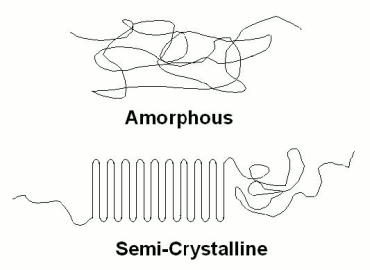
\includegraphics[width=0.4\textwidth]{fig/crystal-1.png}
    \caption{Как цепочки складываются в ламели}
    \label{fig:crystal-1}
  \end{center}
  \vspace{-20pt}
  \vspace{1pt}
\end{wrapfigure}



\begin{figure}[h]
    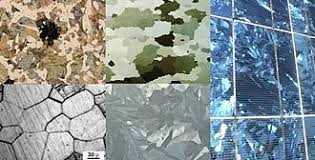
\includegraphics[width=\textwidth]{fig/crystallites.jpg}
    \caption{Типы кристаллитов}
    \label{fig:crystallites}
\end{figure}



\subsection{Частичная кристалличность}

Свойства частичнокристаллических полимеров можно понять, по большей части,
используя простую двухфазную модель, которая предполагает, что две фазы, кристаллическая и аморфная, легко различимы. Если интенсивный параметр  $\phi$ (например, удельный объем) кристаллической и аморфной фазы , $\phi_c$ и $\phi_c$, соответственно, может быть измерен, и мы предполагаем, что вклады двух фаз являются аддитивными, тогда
\[ 
\phi = \phi_c x + \phi_a(1-x),
\]
где $x$  -- доля кристаллической фазы, чаще всего массовая, хотя это в некоторой степени зависит от метода измерения \cite{cryst3}.

Простейшими организованными структурами, образуемыми полимерными цепями, являются кристаллиты, или ламели. Последние делее собираются в фибрилы или сферолиты. Возникновение сферолитов и фибрилл может
используется для определения, является ли полимер кристаллическим или нет, и для измерения локальной кристалличности.

Крупные образования, такие как сферолиты, можно наблюдать с помощью оптической микросопии, в то время как для обнаружения более мелких структур требуются другие методы -- например, электронная микроскопия, атомно-силовая микроскопия и т.д.

	\begin{wrapfigure}{r}{0.5\textwidth} 
\vspace{-20pt}
  \begin{center}
    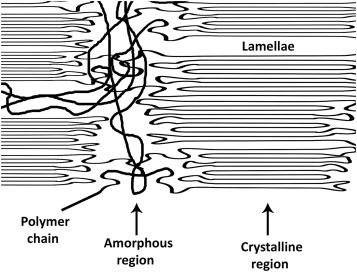
\includegraphics[width=0.4\textwidth]{fig/crystal-2.jpg}
    \caption{К определению кристалличности полимеров}
    \label{fig:crystal-2}
  \end{center}
  \vspace{-20pt}
  \vspace{1pt}
\end{wrapfigure}	

The two-phase model implied in Eq. (3.1) is only an approximation because
there can be a continuum of structures from large, defect-free single crystals to
the truly amorphous domains with liquid-like order. Because of the restrictions
imposed by long polymer chains, defects are invariably present in the crystal lattice,
and the polymer crystallites are small and disordered.\\
Conversely, the amorphous
domains possess some degree of positional and orientational correlations, and there
is experimental evidence for both rigid or ordered and soft or fluid amorphous phases\\
it may not always be possible to distinguish between the signatures
of the crystalline and amorphous phases. Nevertheless, a two-phase model with
an approximate crystalline phase and an amorphous phase, and sometimes an additional
ordered phase, mostly due to oriented amorphous domains, is often used.\\



\subsection{Влияние на макроскопические параметры}





	